% Created by tikzDevice version 0.12.3 on 2020-04-10 11:41:06
% !TEX encoding = UTF-8 Unicode
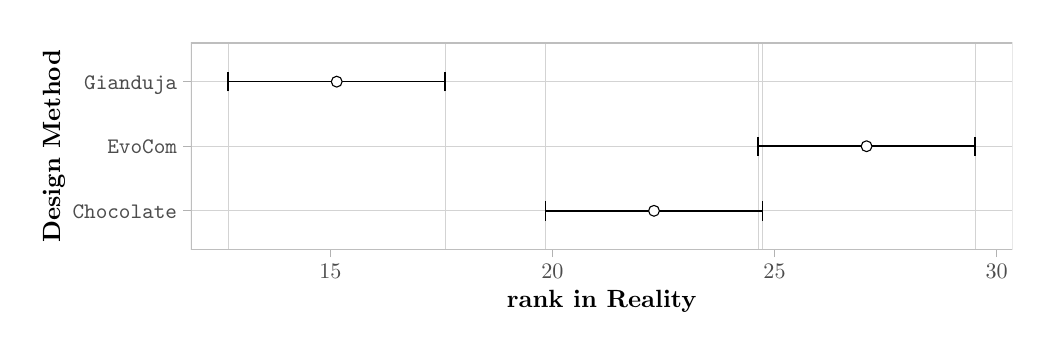
\begin{tikzpicture}[x=1pt,y=1pt]
\definecolor{fillColor}{RGB}{255,255,255}
\path[use as bounding box,fill=fillColor,fill opacity=0.00] (0,0) rectangle (361.35,108.41);
\begin{scope}
\path[clip] (  0.00,  0.00) rectangle (361.35,108.41);
\definecolor{drawColor}{RGB}{255,255,255}
\definecolor{fillColor}{RGB}{255,255,255}

\path[draw=drawColor,line width= 0.6pt,line join=round,line cap=round,fill=fillColor] (  0.00,  0.00) rectangle (361.35,108.41);
\end{scope}
\begin{scope}
\path[clip] ( 58.95, 28.23) rectangle (355.85,102.91);
\definecolor{fillColor}{RGB}{255,255,255}

\path[fill=fillColor] ( 58.95, 28.23) rectangle (355.85,102.91);
\definecolor{drawColor}{RGB}{211,211,211}

\path[draw=drawColor,line width= 0.3pt,line join=round] ( 58.95, 65.57) --
	(355.85, 65.57);

\path[draw=drawColor,line width= 0.3pt,line join=round] ( 58.95, 88.90) --
	(355.85, 88.90);

\path[draw=drawColor,line width= 0.3pt,line join=round] ( 58.95, 42.23) --
	(355.85, 42.23);

\path[draw=drawColor,line width= 0.2pt,line join=round] (265.54, 28.23) -- (265.54,102.91);

\path[draw=drawColor,line width= 0.2pt,line join=round] (342.35, 28.23) -- (342.35,102.91);

\path[draw=drawColor,line width= 0.2pt,line join=round] (150.89, 28.23) -- (150.89,102.91);

\path[draw=drawColor,line width= 0.2pt,line join=round] (187.10, 28.23) -- (187.10,102.91);

\path[draw=drawColor,line width= 0.2pt,line join=round] (263.91, 28.23) -- (263.91,102.91);

\path[draw=drawColor,line width= 0.2pt,line join=round] ( 72.45, 28.23) -- ( 72.45,102.91);
\definecolor{drawColor}{RGB}{0,0,0}

\path[draw=drawColor,line width= 0.6pt,line join=round] (265.54, 38.73) --
	(265.54, 45.73);

\path[draw=drawColor,line width= 0.6pt,line join=round] (265.54, 42.23) --
	(187.10, 42.23);

\path[draw=drawColor,line width= 0.6pt,line join=round] (187.10, 38.73) --
	(187.10, 45.73);

\path[draw=drawColor,line width= 0.6pt,line join=round] (342.35, 62.06) --
	(342.35, 69.07);

\path[draw=drawColor,line width= 0.6pt,line join=round] (342.35, 65.57) --
	(263.91, 65.57);

\path[draw=drawColor,line width= 0.6pt,line join=round] (263.91, 62.06) --
	(263.91, 69.07);

\path[draw=drawColor,line width= 0.6pt,line join=round] (150.89, 85.40) --
	(150.89, 92.40);

\path[draw=drawColor,line width= 0.6pt,line join=round] (150.89, 88.90) --
	( 72.45, 88.90);

\path[draw=drawColor,line width= 0.6pt,line join=round] ( 72.45, 85.40) --
	( 72.45, 92.40);

\path[draw=drawColor,line width= 0.4pt,line join=round,line cap=round,fill=fillColor] (226.32, 42.23) circle (  1.96);

\path[draw=drawColor,line width= 0.4pt,line join=round,line cap=round,fill=fillColor] (303.13, 65.57) circle (  1.96);

\path[draw=drawColor,line width= 0.4pt,line join=round,line cap=round,fill=fillColor] (111.67, 88.90) circle (  1.96);
\definecolor{drawColor}{RGB}{190,190,190}

\path[draw=drawColor,line width= 0.6pt,line join=round,line cap=round] ( 58.95, 28.23) rectangle (355.85,102.91);
\end{scope}
\begin{scope}
\path[clip] (  0.00,  0.00) rectangle (361.35,108.41);
\definecolor{drawColor}{gray}{0.30}

\node[text=drawColor,anchor=base east,inner sep=0pt, outer sep=0pt, scale=  0.80] at ( 54.00, 62.81) {\texttt{EvoCom}};

\node[text=drawColor,anchor=base east,inner sep=0pt, outer sep=0pt, scale=  0.80] at ( 54.00, 86.15) {\texttt{Gianduja}};

\node[text=drawColor,anchor=base east,inner sep=0pt, outer sep=0pt, scale=  0.80] at ( 54.00, 39.47) {\texttt{Chocolate}};
\end{scope}
\begin{scope}
\path[clip] (  0.00,  0.00) rectangle (361.35,108.41);
\definecolor{drawColor}{gray}{0.70}

\path[draw=drawColor,line width= 0.3pt,line join=round] ( 56.20, 65.57) --
	( 58.95, 65.57);

\path[draw=drawColor,line width= 0.3pt,line join=round] ( 56.20, 88.90) --
	( 58.95, 88.90);

\path[draw=drawColor,line width= 0.3pt,line join=round] ( 56.20, 42.23) --
	( 58.95, 42.23);
\end{scope}
\begin{scope}
\path[clip] (  0.00,  0.00) rectangle (361.35,108.41);
\definecolor{drawColor}{gray}{0.70}

\path[draw=drawColor,line width= 0.3pt,line join=round] (109.38, 25.48) --
	(109.38, 28.23);

\path[draw=drawColor,line width= 0.3pt,line join=round] (189.63, 25.48) --
	(189.63, 28.23);

\path[draw=drawColor,line width= 0.3pt,line join=round] (269.88, 25.48) --
	(269.88, 28.23);

\path[draw=drawColor,line width= 0.3pt,line join=round] (350.14, 25.48) --
	(350.14, 28.23);
\end{scope}
\begin{scope}
\path[clip] (  0.00,  0.00) rectangle (361.35,108.41);
\definecolor{drawColor}{gray}{0.30}

\node[text=drawColor,anchor=base,inner sep=0pt, outer sep=0pt, scale=  0.80] at (109.38, 17.77) {15};

\node[text=drawColor,anchor=base,inner sep=0pt, outer sep=0pt, scale=  0.80] at (189.63, 17.77) {20};

\node[text=drawColor,anchor=base,inner sep=0pt, outer sep=0pt, scale=  0.80] at (269.88, 17.77) {25};

\node[text=drawColor,anchor=base,inner sep=0pt, outer sep=0pt, scale=  0.80] at (350.14, 17.77) {30};
\end{scope}
\begin{scope}
\path[clip] (  0.00,  0.00) rectangle (361.35,108.41);
\definecolor{drawColor}{RGB}{0,0,0}

\node[text=drawColor,anchor=base,inner sep=0pt, outer sep=0pt, scale=  0.90] at (207.40,  7.25) {\bfseries rank in Reality};
\end{scope}
\begin{scope}
\path[clip] (  0.00,  0.00) rectangle (361.35,108.41);
\definecolor{drawColor}{RGB}{0,0,0}

\node[text=drawColor,rotate= 90.00,anchor=base,inner sep=0pt, outer sep=0pt, scale=  0.90] at ( 11.71, 65.57) {\bfseries Design Method};
\end{scope}
\end{tikzpicture}
